\section{Experiment with Pozyx}
In order to determine the accuracy of the Pozyx tags we conducted an experiment.
The primary goal of the experiment was to test the accuracy, but a by-product of the experiment was to determine the frequencies of updates for each tag.

\subsection{Setup}
The current settings aims to achieve best precision, but gives a smaller amount of updates.
% Uddyb hvilke settings det er og angiv kilde.
The experiment was setup as shown on \autoref{fig:experiment-setup}. 
The experiment was conducted indoors in Novi 9. 
The anchors \texttt{0x632b} and \texttt{0x676e} were mounted on a wall 240 centimeters apart, and the remaining anchors \texttt{0x6738} and \texttt{0x676c} were mounted on a bulletin board.
The number of centimeters accompanying the hexadecimal number of each anchor is the height at which the anchor was mounted during the experiment.
Different heights were chosen as Pozyx documentation suggests that not all anchors should have the same height \cite{pozyx-AnchorHeights}.
The reason for this is the principle of geometric dilution of precision(GDOP), which can cause the error on range measurements to be amplified.

\begin{figure}[H]
    \centering
    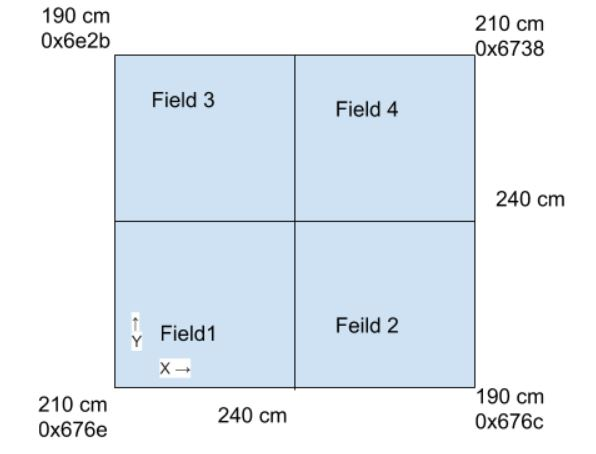
\includegraphics[width=0.6\linewidth]{experiment-setup.JPG}
    \caption{The setup of the experiment with the anchors and the height at which they were placed in the corners.}
    \label{fig:experiment-setup}
\end{figure}
\noindent
The fields were created by a blackboard on which lines were drawn every 10 centimeters to know the actual position as seen on \autoref{fig:experiment-blackboard}.
This blackboard was moved intermittently to act as respectively field 1, field 2, field 3 and field 4.

\begin{figure}[H]
    \centering
    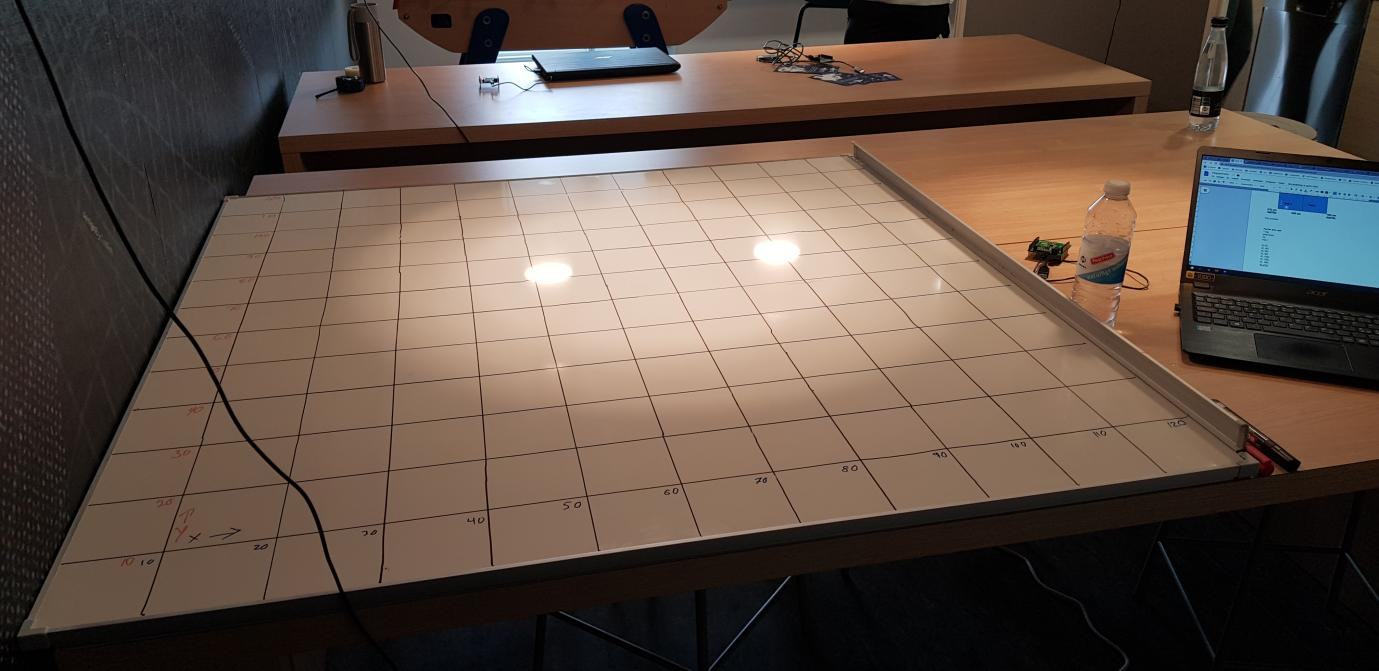
\includegraphics[width=0.8\linewidth]{experiment-blackboard.png}
    \caption{The blackboard with the drawn positions.}
    \label{fig:experiment-blackboard}
\end{figure}
\noindent
The procedure for the experiment was based on this blackboard.
The blackboard would be placed in one of the fields defined in \autoref{fig:experiment-setup}, and we would then place the tags in certain positions on the board and record the accuracy with with the position was reported.
The tags would be placed in a position, remain there for five seconds, then be moved to the next position over the next five seconds and remain in this position for five seconds before being moved again.
This procedure was repeated until a satisfactory number of measurements had been made.
Once one field had been tested, we moved the blackboard to the next field and repeated the setup.
 
\subsection{Precision with 1 tag} \label{sec:one-tag-precision}
As can be seen on \autoref{app:one-tag}

\paragraph{Update frequency}

\subsection{Precision with 3 tag}

24622 was sometimes fairly inaccurate due to there sometimes being few position updates. 
A few times there were no updates in a 2 seconds time spand.    

\paragraph{Update frequency}

\subsection{Precision with 5 tag}

\paragraph{Update frequency}

\subsection{Possible influences on the test}
One thing that could have affected the tags is that we used a blackboard as a measure for positions. 
As there is metal in the blackboard this could have affected the precision on the tags.
Metals are conductors, which can lead to the signal having less power and reduced range, and the signal might spend extra time trying to get through the metal.
Since Pozyx positioning relies on calculating the time of flight, having the signal spend extra time travelling reduces accuracy \cite{pozyx-UWBObstacles}. 
\\\\
During the test with 1 tag, the 0 value of the $x$ coordinate coincided with the wall. 
This could have been an influence on the positing result in that it could increase uncertainty, as it was difficult to center the tag over the x coordinate since the coordinate collided with the wall.

\subsection{Conclusion on the experiment}